\section{Model Definitions}
\label{sec:definitions}
This section presents the definition of the basic components of a stream processing system as
they are used in this work. Many of the concepts are similar or equivalent to their
counterparts already described when presenting the CQL and boxes-and-arrows query models in
Section~\ref{sec:querymod}.
Nevertheless, a precise definition of many concepts used throughout this thesis is necessary for the correct
understanding of this work. Table~\ref{tab:notation} summarises the notation used below.
%--------------------------------------------------------------------------------------------------------
\subsection*{Schema}
In order for the system to be able to interpret the content of a unit of information, it is necessary to
describe the values that it contains, providing a name and a data type for each item. 
Such a definition is contained in a \emph{schema}.
\begin{definition}[Schema]{ 
A schema $S$ is a data structure of elements in the form: $\langle Type, Name \rangle$.}
\end{definition}
A \textit{schema} defines the structure of the payload contained in a tuple. It is formed by a series
of $\langle Type, Name \rangle$ pairs, each specifying the abstract type and the name of an item. It
is equivalent to a schema used in a relational database, where it is used to describe the columns forming a
table. 

\underline{\textsc{Example}}: Consider a tuple with the following schema:\\

\begin{table}[th!]
	\centering
	\begin{tabular}{|c||c|} \hline
	%notation & description \\ \hline
	\textit{Integer} 	&	\textsc{NodeID}		\\	\hline
	\textit{Double}		&	\textsc{CpuLoad}	\\	\hline
	\textit{Long}		&	\textsc{UpTime}		\\	\hline
	\end{tabular}
	
	%\caption{Schema of a tuple containing load and uptime information for a specific processing node.}
	\label{table:schema}
\end{table}

It contains information about load and uptime for a specific sensor. Each field has a name so that
it can be referred to when processing the tuple and it includes an abstract type, which will be
translated to a system type once the tuple is instantiated.\\

%--------------------------------------------------------------------------------------------------------
\subsection*{Tuple}
A schema describes the prototype for a data item processed by a stream processing system. 
An instance of a schema containing actual information to be processed is called a \emph{tuple.}

\begin{table}[t!]
\centering
\begin{tabular}{|c||c|} \hline
%notation & description \\ \hline
\multicolumn{2}{|c|}{{\bf Model Notation}} \\ \hline \hline
$t$                     & tuple\\ \hline
%$t_{\tau}$             & generation timestamp of tuple $t$  \\ \hline
$\tau$	           		& tuple timestamp  \\ \hline
%$t_{SIC}$               & \qm value of tuple $t$ \\ \hline
$QM$               		& tuple quality metric value \\ \hline
%$t_{\mathcal{V}}$       & set of schema values of tuple $t$ \\ \hline
$\mathcal{V}$       	& tuple payload \\ \hline
$S$						& abstract stream of tuples \\ \hline
$B$						& batch of tuples \\ \hline
$O$         		    & operator \\ \hline
$f_{op}$                  & operator function \\ \hline
$Q$			            & query \\ \hline
$f_{Q}$                  & query function \\ \hline
$\mathcal{S}$          & set of all sources attached to a query \\ \hline
$\mathcal{T}^{S}$      & source information tuple set  \\ \hline
% %$\mathbb{T}^{S}$       & set of source tuples space \\ \hline
% $*t^{R}$                 & query result tuple  \\ \hline
% $*\mathbb{T}^{R}$        & stream of query result tuples \\ \hline
% $*f$                     & query function \\ \hline
% $*f^{-1}$                & inverse query function \\ \hline
% $*\mathcal{T}_{in}^{o}$  & set of input tuples to operator $o$  \\ \hline
% $*\mathcal{T}_{out}^{o}$ & set of output tuples of operator $o$  \\ \hline
% %\multicolumn{2}{|c|}{{\bf notation for the data streaming system}} \\ \hline \hline
% $*\mathcal{N}$           & set of nodes \\ \hline
% $*\mathcal{Q}$           & set of queries \\ \hline
% $*\mathbb{T}^{R}_{q}$    & stream of result tuples for query $q$\\ \hline
\end{tabular}
\caption{Notation used in the model definitions.\label{table:query}}
\label{tab:notation}
\end{table} % TABLE DEFINITIONS

\begin{definition}[Tuple]{ 
A tuple is an element $t = \langle \tau, QM, \mathcal{V} \rangle$ where $\tau \in T$ is the
timestamp of the element, QM is a quality metric metadata value and 
$\mathcal{V}$ is a set of values defined by a schema $S$.
}
\end{definition}

A \textit{tuple} is the basic information vector in a stream processing system, representing a
single unit of data. In our model, a tuple is composed by three main elements: a
\textit{timestamp}, a \textit{quality metric} and a \textit{payload}.

With timestamp ($\tau$) we mean an temporal indication of when the tuple was produced. This typically is
the time at which the tuple entered the system. In this case, the sources are only concerned with the
production of the raw data and timestamps are assigned by the system as the UTC time at the moment of
input. It is also possible for the timestamp to be set externally, which is useful in case
of synthetic workloads. In this case, the timestamp is determined by an external entity.

In our model, a tuple is always augmented with a \emph{quality} metadata value ($QM$), which is an
indication of the amount of information that is contained in the tuple. This value is maintained by the
system and varies according to the amount of failure (\ie tuple loss) that occurred during the
processing of the tuple.
It has two main functions: it reports back to the user the achieved quality of processing for the
current processing, and it is used internally by the system to make intelligent load-shedding decisions
under overload.

The third element composing a tuple is the \textit{payload} ($\mathcal{V}$). It contains the actual
information carried by the tuple. It is formed by one or more values of any primitive data type. 
The type and the order of the values forming a tuple payload is defined by the schema.

Logically, we can divide tuples in three categories: a \textit{source} tuple ($t_{src}$) is a tuple
generated from a data source representing a single input to the system; a \textit{derived} tuple ($t_{op}
\in \mathcal{T}_{out}^{o}$) is a tuple generated by an intermediate operator; and, finally, there exist
\textit{result} tuples ($t_{res}$), which are derived tuples produced by a terminal operator. They
contains the final results of the processing, which are delivered to the user together with the \qm
value.

\underline{\textsc{Example}}: Figure~\ref{fig:tuple} shows a simple tuple with its relational schema.
It shows a \emph{timestamp} expressed as POSIX time, a \emph{quality metric} value and a \emph{payload}
with three fields carrying information about the CPU load and uptime of a machine monitored by the system.
We discuss the implementation of tuples in Section~\ref{sec:tuples}.
\begin{figure}[t]
	\centering
	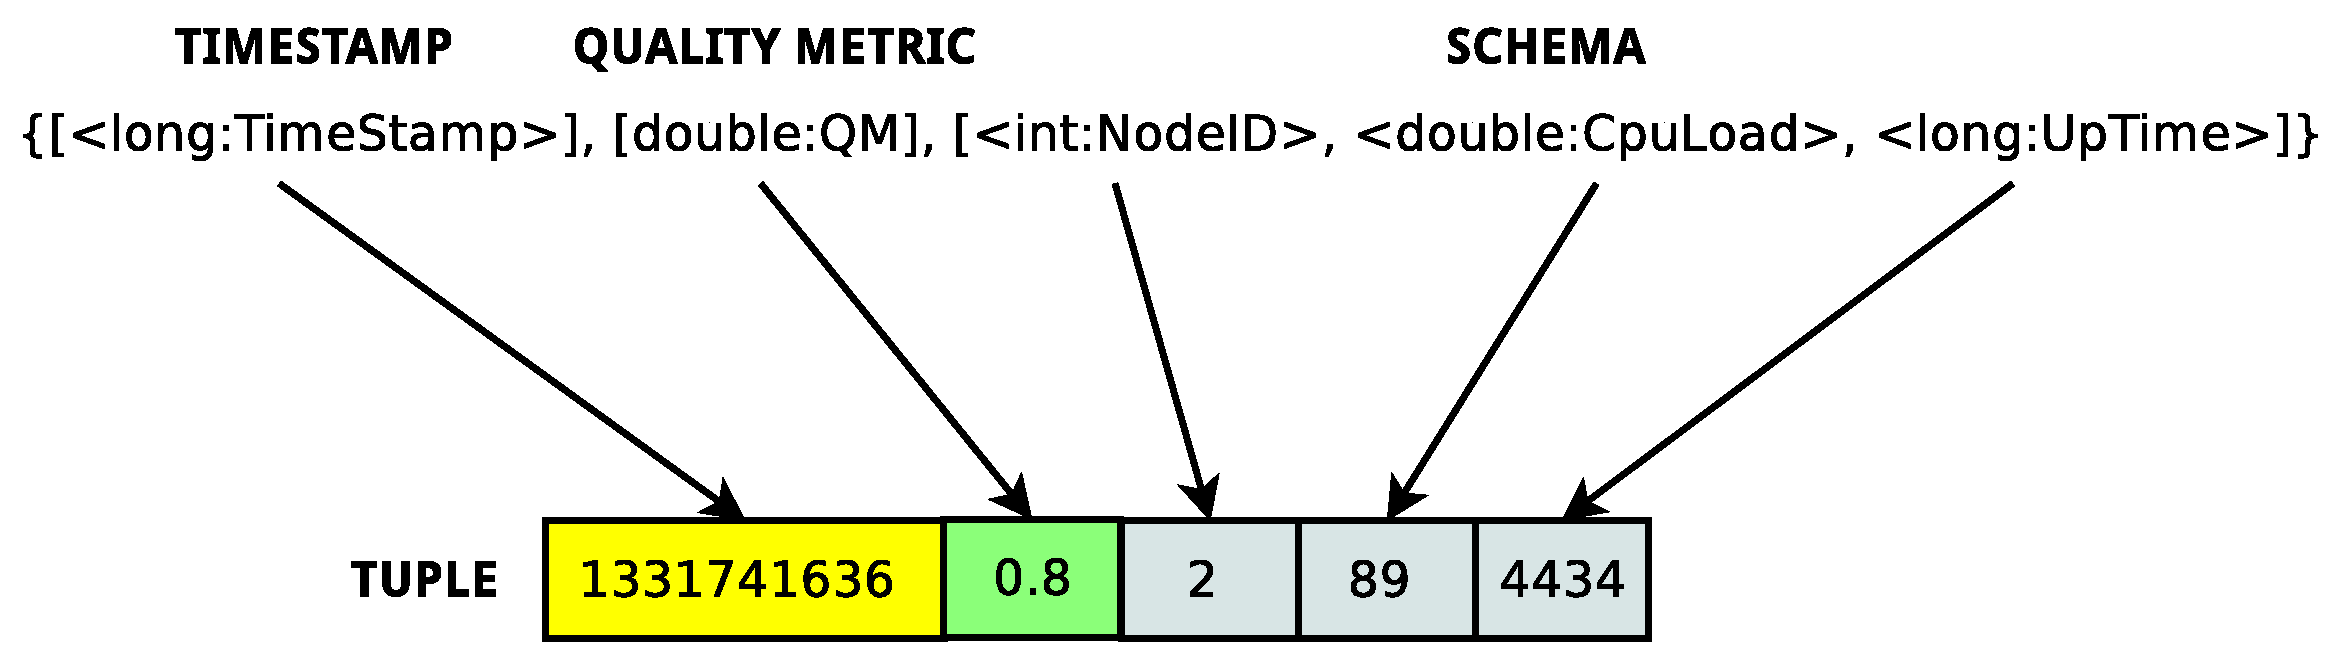
\includegraphics[width=0.8\textwidth]{img/tesi/tuple}
	\caption{A simple tuple with the relational schema.}
	\label{fig:tuple}
\end{figure}
%--------------------------------------------------------------------------------------------------------
\vspace{-10pt}
\subsection*{Stream}
A \emph{stream} is an abstract entity that describes all tuples flowing between two
operators. The number of tuples is potentially infinite and all tuples share a common schema.
\begin{definition}[Stream] {
A stream is a potentially unbounded time-ordered sequence of tuples, all belonging to the same schema.}
\end{definition}
A \textit{stream} is a logical abstraction, representing the totality of the
tuples flowing between two operators. It is time ordered, meaning that a tuple $t_2$ received after a
tuple $t_1$ always has a timestamp greater than or equal to $t_2$ (\ie $\tau_2 \geq \tau_1$).

% We can distinguish between  streams, \textit{derived} streams and \textit{output} streams.
Analogous to tuples, streams can be divided into three categories: \textit{base} streams ($S_{src}$) are
generated from sources and are the input to the system; \emph{derived} streams ($S^{o}_{out}$) are
produced as an output by the operators of a running query; and \emph{result} streams ($S_{res}$) are
derived streams produced by a terminal operator, which contain the results of the processing delivered
to the user.

A stream is used only logically to describe a potentially unbounded sequence of tuples flowing between
two operators. The system, however, needs a finite amount of tuples to operate, which in our system is
represented by a \textit{batch}.

%--------------------------------------------------------------------------------------------------------
\subsection*{Batch}
Streams are continuous abstract entities, while operators need a finite set of tuples to operate.
The system thus partitions streams into \emph{batches}: finite snapshots of a stream, containing
tuples that have the same \emph{quality metric} value to be used as input and output units for
operators.

\begin{definition}[Batch]{
A batch is a finite set of tuples $B=\{t_1,\dots,t_n\}$, all having the same \qm metadata value.
}
\end{definition}

A \textit{batch} is a logical group of tuples with the same quality metric value. In our model, an
operator does not work on a single tuple but on batches. It processes one or more input batches and produces one
output batch, which may be composed of a single tuple.
Using batches allows for a more compact representation of the \qm metadata because it does not have to be
included with each tuple. It also speeds up the calculation of the new \qm value when an operator
outputs a new set of tuples.
 
Batches represent a snapshot of a stream (\ie a finite amount of tuples that can be processed by an
operator). In our system, they are the equivalent to \textit{relations} used in CQL.
The discussion about our implementation of batches is given in Section~\ref{sec:batches}.

%--------------------------------------------------------------------------------------------------------
\vspace{-10pt}
\subsection*{Operator}
A stream processing system transforms a set of input tuples into a set of output tuples representing the
answer to a given query. This data transformation used to produce a result is carried out by a number
of \emph{operators}.


\begin{definition}[Operator]{
An operator is a function $f_{op}$ over a set of input streams $S_{in}=\{S_1,\dots,S_n\}$,
that generates a new output stream $S_{out}$=$f_{op}(S_{in})$. 
}
\end{definition}
 
An \textit{operator} is the basic processing unit in a stream processing system. It represents a
function over a set of input streams, transforming  one or more input batches into one output batch. 

Operators are seen as \textit{black boxes} in our system, meaning that their internal semantic is not
taken into account when calculating the \qm value for the newly generated derived tuples.
We can divide operators based on their behaviour when handling input streams into two categories:
\textit{blocking} or \textit{non-blocking} operators.

Blocking operators need to have at least one input batch available on each of their input
streams. For example, if there are two inputs to an operator, one containing two input
batches while the other one being currently empty, the operator blocks until an
input batch arrives on the second input stream. When this happens, the first batch of each input is removed and processed,
producing one derived batch. Assuming no other batch has arrived on the second input, the operator
blocks again, as only the first input contains data to be processed.

Non-Blocking operators do not need input on all channels to be triggered. Instead, they produce
a derived batch as soon as at least one input batch is present on one of their input channels. 
Such an operator never blocks waiting for input and never has pending input data.
%The discussion about our implementation of queries is given in Section~\ref{sec:queries}.

\begin{figure}[b!]
	\centering
	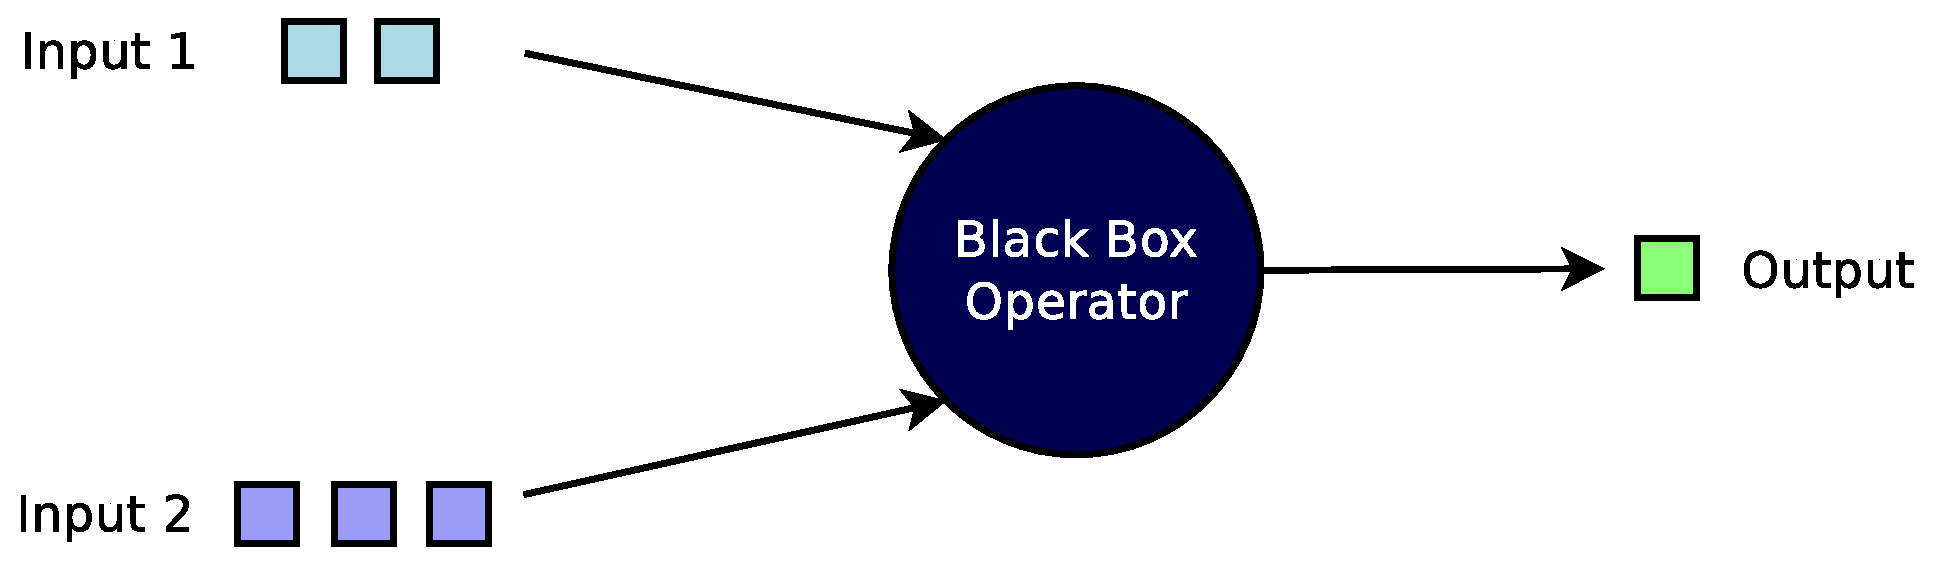
\includegraphics[width=0.7\textwidth]{img/tesi/operator} 
	\caption{A black-box operator with two input and one output stream.}
	\label{fig:tuple}
\end{figure}

%--------------------------------------------------------------------------------------------------------
\vspace{-10pt}
\subsection*{Query}
The processing required to transform the information contained in input tuples into a useful
output for the user is typically not performed by a single operator but by a group of them, arranged into
a logical processing graph. This graph is referred to as a \emph{query}.

 \begin{definition}[Query]{
A query logically defines a series of processing steps over a set of input streams 
$S_{in}=\{S_{in}^1,\dots,S_{in}^n\}$ to produce a desired set of output streams 
$S_{out}=\{S_{out}^1,\dots,S_{out}^n\}$ by the means of a finite number of operators.
}
\end{definition}
%%\mnote{Does it need better definition? How?}

A query describes the processing to transform a set of input streams into a set of output streams.
In the boxes-and-arrows model, queries are depicted as a directed acyclic graph (DAG), in which arcs
represent streams and vertices represent operators. One or more sources produce streams of tuples at
time-varying rates, which are the input to the system. One or more operators process these
tuples, either in sequence or in parallel.

A query is a graph, in which vertices correspond to operators and arcs indicate the direction of tuples
flowing from one or more sources to one or more terminal operators. The set of query operators is
given by $\mathcal{O}$ and cumulatively computes the query function $f_Q$. Operators may be distributed
over a set of nodes $N$ if the query function is too complex to be computed on a single machine.
The discussion about our implementation of queries is given in Section~\ref{sec:queries}.

%--------------------------------------------------------------------------------------------------------
